\section{Vortex Mass as Inertia from Circulation}

In the Vortex Æther Model (VAM), the mass of a knotted vortex is not treated as a fundamental attribute but emerges as a consequence of circulation and resistance to deformation within the æther medium.

\subsection*{Circulation as the Basis for Inertia}

The circulation of a closed vortex path is defined as:
\[
    \Gamma = \oint_{\partial S} \vec{v} \cdot d\vec{\ell} = 2\pi r_c C_e
\]
This quantity is conserved in ideal fluids, as per Helmholtz’s theorems, and serves as a topological invariant of each knot configuration.

Given a fixed $\Gamma$, any change in the vortex core radius $r_c$ must be accompanied by a compensating change in swirl velocity $C_e$:
\[
    C_e = \frac{\Gamma}{2\pi r_c}
\]

\begin{figure}[h!]
    \centering
    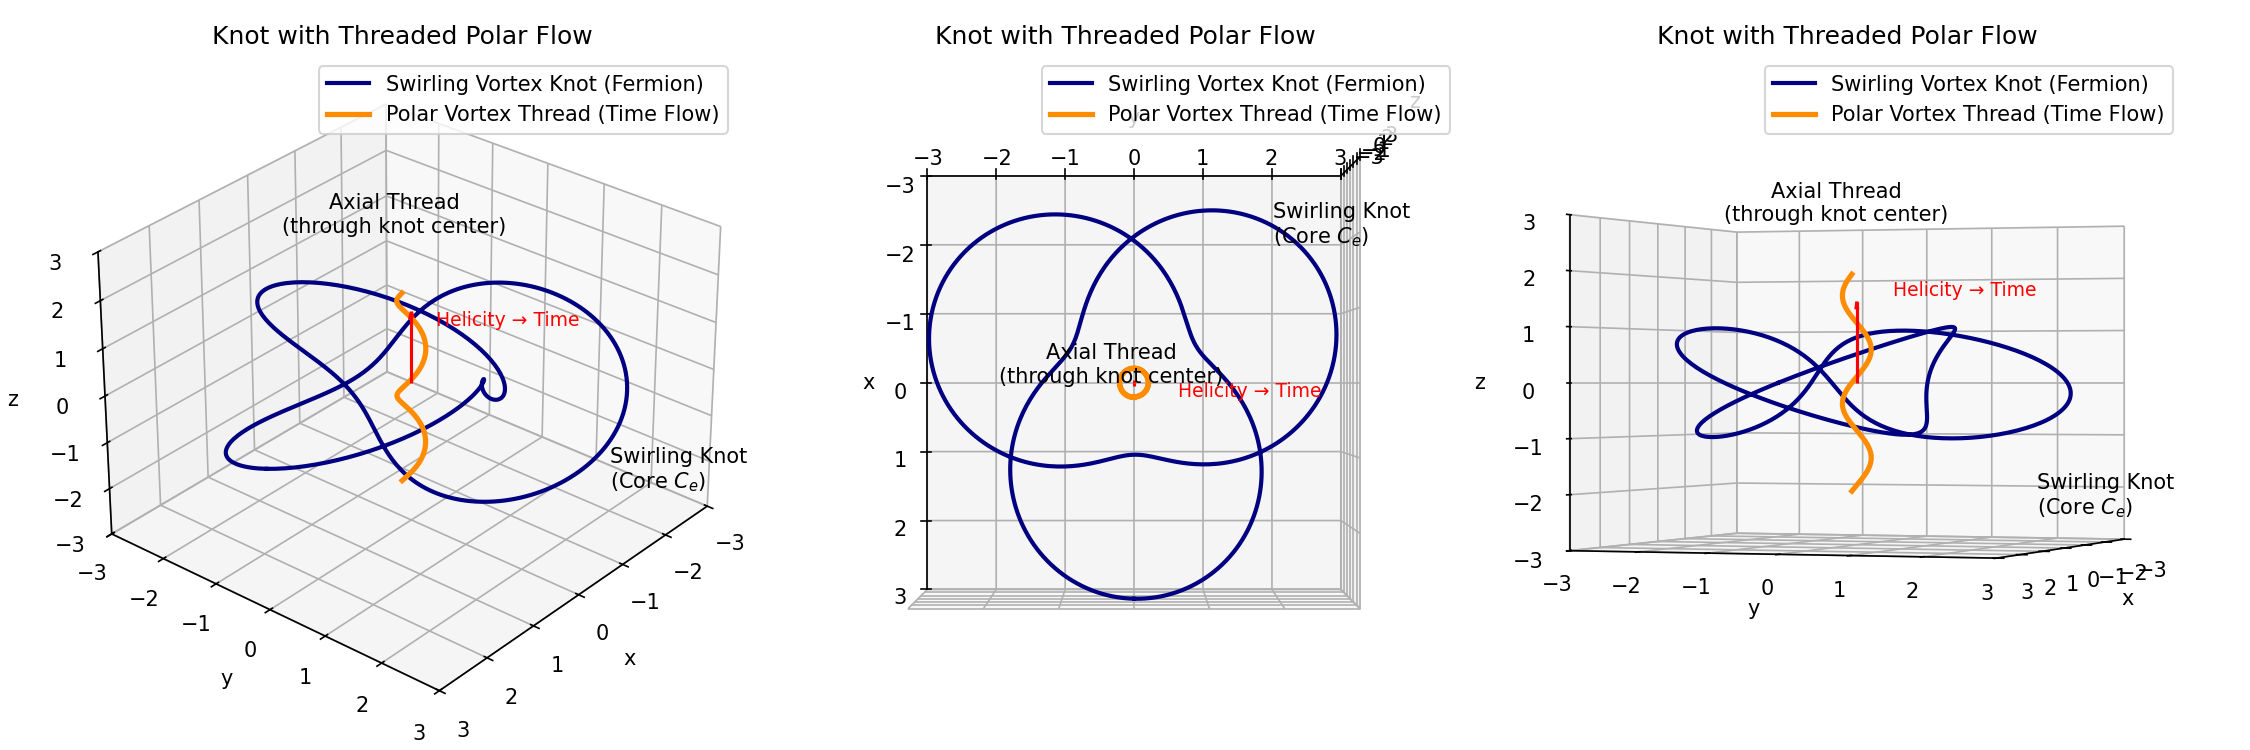
\includegraphics[width=0.98\textwidth]{KnotThreadedPolarFlow.png}
    \caption{Knotted vortex structure linked to a polar thread. Local helicity transports temporal phase.}
\end{figure}

This relation illustrates that the swirl velocity $C_e$ is not arbitrary, but a function of the geometry and topological strength $\Gamma$. Thus, in VAM, mass is not an intrinsic constant—it arises from vortex geometry and the dynamic rigidity of the structure.

\subsection*{Deriving Effective Mass}

The kinetic energy associated with the vortex swirl can be expressed as:
\[
    E = \frac{1}{2} \rho_{\ae} C_e^2 V = \frac{1}{2} \rho_{\ae} \left( \frac{\Gamma}{2\pi r_c} \right)^2 \cdot \frac{4}{3}\pi r_c^3
\]
\[
    \Rightarrow E = \frac{\rho_{\ae} \Gamma^2}{6\pi r_c}
\]

By comparing this expression with the classical inertial energy form $E = \frac{1}{2} m C_e^2$, we extract the effective mass of the vortex:
\[
    m_\text{eff} = \frac{\rho_{\ae} \Gamma^2}{3\pi r_c C_e^2}
\]

This result shows that mass in VAM emerges from:
- The conserved circulation $\Gamma$,
- The knot’s spatial extent $r_c$,
- The internal swirl velocity $C_e$.

\subsection*{Comparison to Classical Inertia}

For comparison, standard relativity yields:
\[
    m \sim \frac{E}{c^2} \quad \text{vs.} \quad E = \frac{1}{2} m C_e^2 \quad \text{in VAM}
\]
Here, $C_e$ represents the local internal swirl constant, while $c$ is the emergent propagation speed of disturbances. Thus, mass in VAM is not postulated as fundamental but is fully derivable from geometric and conservation principles.

\subsection*{Fermion Mass Term in the Lagrangian}

From this derivation, the fermion mass term in the VAM Lagrangian can be written as:
\[
    \mathcal{L}_\text{mass} = m_f C_e r_c \cdot \bar{\psi}_f \psi_f
\]
where $m_f$ is proportional to the æther density $\rho_{\ae}$ and circulation strength $\Gamma^2$ of the vortex knot. This replaces the conventional Yukawa coupling with a fluid-mechanical origin of mass.
